\documentclass[]{article}
\usepackage{lmodern}
\usepackage{amssymb,amsmath}
\usepackage{ifxetex,ifluatex}
\usepackage{fixltx2e} % provides \textsubscript
\ifnum 0\ifxetex 1\fi\ifluatex 1\fi=0 % if pdftex
  \usepackage[T1]{fontenc}
  \usepackage[utf8]{inputenc}
\else % if luatex or xelatex
  \ifxetex
    \usepackage{mathspec}
  \else
    \usepackage{fontspec}
  \fi
  \defaultfontfeatures{Ligatures=TeX,Scale=MatchLowercase}
\fi
% use upquote if available, for straight quotes in verbatim environments
\IfFileExists{upquote.sty}{\usepackage{upquote}}{}
% use microtype if available
\IfFileExists{microtype.sty}{%
\usepackage{microtype}
\UseMicrotypeSet[protrusion]{basicmath} % disable protrusion for tt fonts
}{}
\usepackage[margin=1in]{geometry}
\usepackage{hyperref}
\hypersetup{unicode=true,
            pdftitle={Predicting Real Estate Sales Using Machine Learning and Spatial Dependence},
            pdfborder={0 0 0},
            breaklinks=true}
\urlstyle{same}  % don't use monospace font for urls
\usepackage{color}
\usepackage{fancyvrb}
\newcommand{\VerbBar}{|}
\newcommand{\VERB}{\Verb[commandchars=\\\{\}]}
\DefineVerbatimEnvironment{Highlighting}{Verbatim}{commandchars=\\\{\}}
% Add ',fontsize=\small' for more characters per line
\usepackage{framed}
\definecolor{shadecolor}{RGB}{248,248,248}
\newenvironment{Shaded}{\begin{snugshade}}{\end{snugshade}}
\newcommand{\KeywordTok}[1]{\textcolor[rgb]{0.13,0.29,0.53}{\textbf{#1}}}
\newcommand{\DataTypeTok}[1]{\textcolor[rgb]{0.13,0.29,0.53}{#1}}
\newcommand{\DecValTok}[1]{\textcolor[rgb]{0.00,0.00,0.81}{#1}}
\newcommand{\BaseNTok}[1]{\textcolor[rgb]{0.00,0.00,0.81}{#1}}
\newcommand{\FloatTok}[1]{\textcolor[rgb]{0.00,0.00,0.81}{#1}}
\newcommand{\ConstantTok}[1]{\textcolor[rgb]{0.00,0.00,0.00}{#1}}
\newcommand{\CharTok}[1]{\textcolor[rgb]{0.31,0.60,0.02}{#1}}
\newcommand{\SpecialCharTok}[1]{\textcolor[rgb]{0.00,0.00,0.00}{#1}}
\newcommand{\StringTok}[1]{\textcolor[rgb]{0.31,0.60,0.02}{#1}}
\newcommand{\VerbatimStringTok}[1]{\textcolor[rgb]{0.31,0.60,0.02}{#1}}
\newcommand{\SpecialStringTok}[1]{\textcolor[rgb]{0.31,0.60,0.02}{#1}}
\newcommand{\ImportTok}[1]{#1}
\newcommand{\CommentTok}[1]{\textcolor[rgb]{0.56,0.35,0.01}{\textit{#1}}}
\newcommand{\DocumentationTok}[1]{\textcolor[rgb]{0.56,0.35,0.01}{\textbf{\textit{#1}}}}
\newcommand{\AnnotationTok}[1]{\textcolor[rgb]{0.56,0.35,0.01}{\textbf{\textit{#1}}}}
\newcommand{\CommentVarTok}[1]{\textcolor[rgb]{0.56,0.35,0.01}{\textbf{\textit{#1}}}}
\newcommand{\OtherTok}[1]{\textcolor[rgb]{0.56,0.35,0.01}{#1}}
\newcommand{\FunctionTok}[1]{\textcolor[rgb]{0.00,0.00,0.00}{#1}}
\newcommand{\VariableTok}[1]{\textcolor[rgb]{0.00,0.00,0.00}{#1}}
\newcommand{\ControlFlowTok}[1]{\textcolor[rgb]{0.13,0.29,0.53}{\textbf{#1}}}
\newcommand{\OperatorTok}[1]{\textcolor[rgb]{0.81,0.36,0.00}{\textbf{#1}}}
\newcommand{\BuiltInTok}[1]{#1}
\newcommand{\ExtensionTok}[1]{#1}
\newcommand{\PreprocessorTok}[1]{\textcolor[rgb]{0.56,0.35,0.01}{\textit{#1}}}
\newcommand{\AttributeTok}[1]{\textcolor[rgb]{0.77,0.63,0.00}{#1}}
\newcommand{\RegionMarkerTok}[1]{#1}
\newcommand{\InformationTok}[1]{\textcolor[rgb]{0.56,0.35,0.01}{\textbf{\textit{#1}}}}
\newcommand{\WarningTok}[1]{\textcolor[rgb]{0.56,0.35,0.01}{\textbf{\textit{#1}}}}
\newcommand{\AlertTok}[1]{\textcolor[rgb]{0.94,0.16,0.16}{#1}}
\newcommand{\ErrorTok}[1]{\textcolor[rgb]{0.64,0.00,0.00}{\textbf{#1}}}
\newcommand{\NormalTok}[1]{#1}
\usepackage{graphicx,grffile}
\makeatletter
\def\maxwidth{\ifdim\Gin@nat@width>\linewidth\linewidth\else\Gin@nat@width\fi}
\def\maxheight{\ifdim\Gin@nat@height>\textheight\textheight\else\Gin@nat@height\fi}
\makeatother
% Scale images if necessary, so that they will not overflow the page
% margins by default, and it is still possible to overwrite the defaults
% using explicit options in \includegraphics[width, height, ...]{}
\setkeys{Gin}{width=\maxwidth,height=\maxheight,keepaspectratio}
\IfFileExists{parskip.sty}{%
\usepackage{parskip}
}{% else
\setlength{\parindent}{0pt}
\setlength{\parskip}{6pt plus 2pt minus 1pt}
}
\setlength{\emergencystretch}{3em}  % prevent overfull lines
\providecommand{\tightlist}{%
  \setlength{\itemsep}{0pt}\setlength{\parskip}{0pt}}
\setcounter{secnumdepth}{0}
% Redefines (sub)paragraphs to behave more like sections
\ifx\paragraph\undefined\else
\let\oldparagraph\paragraph
\renewcommand{\paragraph}[1]{\oldparagraph{#1}\mbox{}}
\fi
\ifx\subparagraph\undefined\else
\let\oldsubparagraph\subparagraph
\renewcommand{\subparagraph}[1]{\oldsubparagraph{#1}\mbox{}}
\fi

%%% Use protect on footnotes to avoid problems with footnotes in titles
\let\rmarkdownfootnote\footnote%
\def\footnote{\protect\rmarkdownfootnote}

%%% Change title format to be more compact
\usepackage{titling}

% Create subtitle command for use in maketitle
\newcommand{\subtitle}[1]{
  \posttitle{
    \begin{center}\large#1\end{center}
    }
}

\setlength{\droptitle}{-2em}
  \title{Predicting Real Estate Sales Using Machine Learning and Spatial
Dependence}
  \pretitle{\vspace{\droptitle}\centering\huge}
  \posttitle{\par}
  \author{}
  \preauthor{}\postauthor{}
  \date{}
  \predate{}\postdate{}

\setlength{\parindent}{4em}
\setlength{\parskip}{0em}

\begin{document}
\maketitle

{
\setcounter{tocdepth}{2}
\tableofcontents
}
\section{Introduction}\label{introduction}

\subsection{Motivating Example: Combatting Economic
Exclusion}\label{motivating-example-combatting-economic-exclusion}

Predictive modeling using spatial dependence has been employed
extensively in recent years, notably in Crime Prediction (Almanie 2015).
However, a key deficiency of many spatial models are their use of
arbitrarily defined geographic regions, such as zip codes, political
districts, police precincts, state lines, neighborhoods, etc. which
diminish and obscure potentially valuable insights. Worse yet, many
predictive models ignore and exclude spatial dependence, violating one
of the basic tenets of geography: the direct relationship between
distance and likeness (Miller 2007).

Income inequality may be a central challenge of our time. Researchers at
the Urban Institute (Solomon Greene and Lei 2016) recently identified
the socio-economic phenomenon of ``Economic Exclusion'' as one
compelling explanation for the recent rise in inequality in the US.
Vulnerable populations (disproportionately communities of color,
immigrants, refugees, and women), who are displaced by localized
economic prosperity enter into a gradual cycle of diminished access to
good jobs, good schools, health care facilities, public spaces, etc.
This systematic denial causes enduring and self-reinforcing poverty over
the course years and even generations, gradually entrenching income
inequality and general unrest.

One way to practically combat economic exclusion is to focus on
preventing displacement, however, detecting gentrification at an early
enough stage can be a daunting task. When an area experiences economic
growth, increased housing demands and subsequent affordability pressures
can lead to evictions of low-income families and small businesses.
Government agencies and nonprofits tend to intervene once displacement
is already underway, and after-the-fact interventions can be costly and
ineffective. There are a host of pre-emptive actions that can be
deployed to stem divestment and ensure that existing residents benefit
from new investments. Not unlike medical treatment, early detection is
key to success. Consequently, in 2016, the Urban Institute put forth a
call for research into the creation of ``neighborhood-level early
warning and response systems that can help city leaders and community
advocates get ahead of neighborhood changes'' (2016).

This paper explores novel techniques to predict gentrification in the
pursuit of combating displacement and economic exclusion. Modern
techniques of data mining, machine learning and predictive modeling are
applied to datasets describing property values and sale prices in New
York City. We explore the viability of using spatial lags, i.e.,
variables created from physically proximate observations, as features in
a machine learning predictive model.

\subsection{Geo-spatial Data}\label{geo-spatial-data}

The world has seen an unprecedented amount of geospatial data produced
in recent years (i.e., data that contain information about where an
observation exists or happened). Every day in the U.S., federal, state
and local government agencies are making their troves of geo-spatially
tagged data available for the benefit of the public. Adequate tools to
describe, explore and model such data are in short supply for the
data-journalists and data-activists who have become modern mechanisms of
public service. It is imperative that research be done and tools created
to better harness such data for commercial and public good.

\section{Literature Review}\label{literature-review}

\subsection{Lit Review}\label{lit-review}

Much of the research on predicting real estate values has been in
service of creating mass appraisal models. Mass appraisal models share
many characteristics with predictive machine learning model modeling,
primarily in that they are data-driven, standardized methods that employ
statistical testing (Eckert 1990).

\subsection{sample citations}\label{sample-citations}

Sample Citation: (Antipov and Pokryshevskaya 2012) (see: Antipov and
Pokryshevskaya 2012, 33--35; also Antipov and Pokryshevskaya 2012, ch.~1
and \emph{passim})

A minus sign (-) before the @ will suppress mention of the author in the
citation. This can be useful when the author is already mentioned in the
text:

Antipov says blah (2012).

You can also write an in-text citation, as follows:

Antipov and Pokryshevskaya (2012) says blah.

\section{Methodology}\label{methodology}

\subsection{Methodology Section}\label{methodology-section}

Random Forrest has several advantages over traditional geographic
weighted regression, amoung them:

\begin{enumerate}
\def\labelenumi{\arabic{enumi}.}
\tightlist
\item
  Ability to handle large amounts of categorical data without much
  pre-processing
\item
  Ability to model in spite of missing values in data
\item
  Eliminated colinearity as a concern
\item
  Allows for the introduction of many more variables without requiring
  penalty for additional predictors
\item
  Works relatively fast and can be parallelized
\end{enumerate}

\section{Results}\label{results}

\begin{Shaded}
\begin{Highlighting}[]
\KeywordTok{plot}\NormalTok{(mtcars}\OperatorTok{$}\NormalTok{wt, mtcars}\OperatorTok{$}\NormalTok{mpg, }\DataTypeTok{col =}\NormalTok{ mtcars}\OperatorTok{$}\NormalTok{cyl)}
\end{Highlighting}
\end{Shaded}

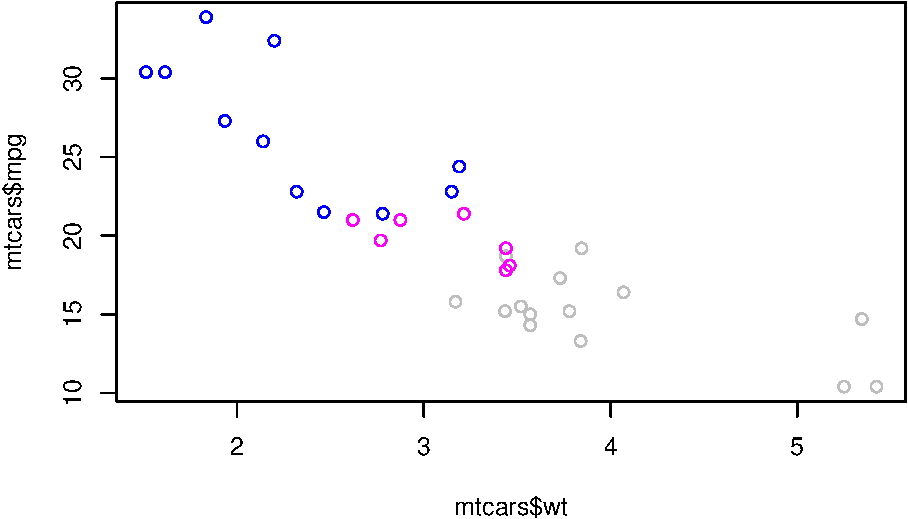
\includegraphics{Thesis_files/figure-latex/unnamed-chunk-6-1.pdf}

Note that the \texttt{echo\ =\ FALSE} parameter was added to the code
chunk to prevent printing of the R code that generated the plot.

\section{Conclusions and Future
Research}\label{conclusions-and-future-research}

\begin{Shaded}
\begin{Highlighting}[]
\KeywordTok{plot}\NormalTok{(pressure}\OperatorTok{$}\NormalTok{temperature, pressure}\OperatorTok{$}\NormalTok{pressure)}
\end{Highlighting}
\end{Shaded}

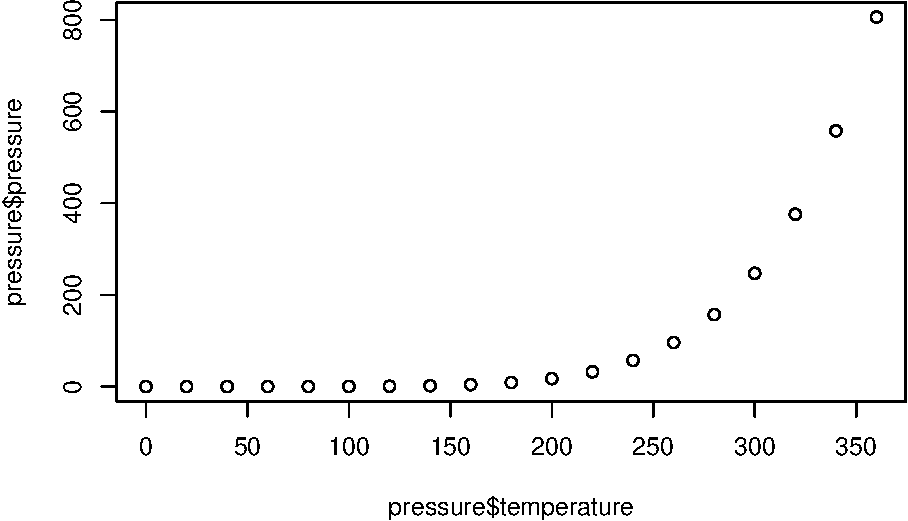
\includegraphics{Thesis_files/figure-latex/unnamed-chunk-7-1.pdf}

Note that the \texttt{echo\ =\ FALSE} parameter was added to the code
chunk to prevent printing of the R code that generated the plot.

\section*{References}\label{references}
\addcontentsline{toc}{section}{References}

\hypertarget{refs}{}
\hypertarget{ref-Almanie2015}{}
Almanie, R.; Lor, T.; Mirza. 2015. ``Crime Prediction Based on Crime
Types and Using Spatial and Temporal Criminal Hotspots.''
\emph{International Journal of Data Mining \& Knowledge Management
Process (IJDKP)} 5 (4).

\hypertarget{ref-antipov12}{}
Antipov, Evgeny A., and Elena B. Pokryshevskaya. 2012. ``Mass Appraisal
of Residential Apartments: An Application of Random Forest for Valuation
and a Cart-Based Approach for Model Diagnostics.'' \emph{Expert Systems
with Applications}.

\hypertarget{ref-Eckert1990}{}
Eckert, J. K. 1990. \emph{Property Appraisal and Assessment
Administration}. Chicago, IL.: International Association of Assessing
Officers.

\hypertarget{ref-Miller2015}{}
Miller, J.; Aspinall, J.; Franklin. 2007. ``Incorporating Spatial
Dependence in Predictive Vegetation Models.'' \emph{Ecological
Modelling} 202 (3): 225--42.

\hypertarget{ref-urban2016}{}
Solomon Greene, Molly Scott, Rolf Pendall, and Serena Lei. 2016. ``Open
Cities: From Economic Exclusion to Urban Inclusion.'' \emph{Urban
Institue Brief}, June. Urban Institue Brief.


\end{document}
